\documentclass{article}
\usepackage{booktabs}
\usepackage{multirow}
\usepackage{multicol}
\usepackage[table]{xcolor}
\usepackage{colortbl}
\usepackage[backend=biber,natbib=true,style=alphabetic,maxbibnames=50]{biblatex}
\addbibresource{/home/nqbh/reference/bib.bib}
\usepackage[utf8]{vietnam}
\usepackage{tocloft}
\usepackage{tcolorbox}

\setlength{\parindent}{0pt}


\usepackage{minted}

\usepackage{listings}
\usepackage{xcolor}

\lstset{
    language=C++,                    % Ngôn ngữ lập trình
    basicstyle=\ttfamily\footnotesize, % Cỡ chữ nhỏ hơn
    keywordstyle=\color{blue},        % Màu từ khóa
    commentstyle=\color{gray},        % Màu chú thích
    stringstyle=\color{red},          % Màu chuỗi ký tự
    numbers=left,                     % Hiển thị số dòng bên trái
    numberstyle=\tiny\color{gray},    % Định dạng số dòng
    stepnumber=1,                     % Mỗi dòng đều có số dòng
    breaklines=true,                   % Tự động xuống dòng nếu quá dài
    frame=single                      % Đóng khung mã nguồn
}

\renewcommand{\cftsecleader}{\cftdotfill{\cftdotsep}}
\usepackage[colorlinks=true,linkcolor=blue,urlcolor=red,citecolor=magenta]{hyperref}
\usepackage{amsmath,amssymb,amsthm,enumitem,float,graphicx,mathtools,tikz}
\usetikzlibrary{angles,calc,intersections,matrix,patterns,quotes,shadings}
\allowdisplaybreaks
\newtheorem{assumption}{Assumption}
\newtheorem{baitoan}{}
\newtheorem{cauhoi}{Câu hỏi}
\newtheorem{conjecture}{Conjecture}
\newtheorem{corollary}{Corollary}
\newtheorem{dangtoan}{Dạng toán}
\newtheorem{definition}{Definition}
\newtheorem{dinhly}{Định lý}
\newtheorem{dinhnghia}{Định nghĩa}
\newtheorem{example}{Example}
\newtheorem{ghichu}{Ghi chú}
\newtheorem{hequa}{Hệ quả}
\newtheorem{hypothesis}{Hypothesis}
\newtheorem{lemma}{Lemma}
\newtheorem{luuy}{Lưu ý}
\newtheorem{nhanxet}{Nhận xét}
\newtheorem{notation}{Notation}
\newtheorem{note}{Note}
\newtheorem{principle}{Principle}
\newtheorem{problem}{Problem}
\newtheorem{proposition}{Proposition}
\newtheorem{question}{Question}
\newtheorem{remark}{Remark}
\newtheorem{theorem}{Theorem}
\newtheorem{vidu}{Ví dụ}
\usepackage[left=1cm,right=1cm,top=5mm,bottom=5mm,footskip=4mm]{geometry}
\def\labelitemii{$\circ$}
\DeclareRobustCommand{\divby}{%
	\mathrel{\vbox{\baselineskip.65ex\lineskiplimit0pt\hbox{.}\hbox{.}\hbox{.}}}%
}
\setlist[itemize]{leftmargin=*}
\setlist[enumerate]{leftmargin=*}

\title{CHUYÊN ĐỀ: QUY HOẠCH ĐỘNG (DYNAMIC PROGRAMMING)} 
\author{Đặng Phúc An Khang\footnote{ E-mail: {\tt ankhangluonvuituoi@gmail.com}. Tây Ninh, Việt Nam.}}
\date{\today}

\begin{document}
\maketitle
\begin{abstract}
	
	
	\textbf{Code:}
	\begin{quote}
		\begin{itemize}
			\item C{\tt/}C++: \url{https://github.com/GrootTheDeveloper/OLP-ICPC/tree/master/2025/C%2B%2B}.
			\item Python: \url{}\\
		\end{itemize}
	\end{quote}
	
	\textbf{Tài khoản trên các Online Judge:}
	\begin{quote}
    	\begin{itemize}
			\item Codeforces: \url{https://codeforces.com/profile/vuivethoima}.
			\item VNOI: \url{oj.vnoi.info/user/Groot}.
			\item IUHCoder: \url{oj.iuhcoder.com/user/ankhang2111}.
			\item MarisaOJ: \url{https://marisaoj.com/user/grootsiuvip/submissions}.
			\item CSES: \url{https://cses.fi/user/212174}.
			\item UMTOJ: \url{sot.umtoj.edu.vn/user/grootsiuvip}.
			\item SPOJ: \url{www.spoj.com/users/grootsiuvip/}.
			\item POJ: \url{http://poj.org/userstatus?user_id=vuivethoima}.
			\item ATCoder: \url{https://atcoder.jp/users/grootsiuvip}
			\item OnlineJudge.org: \url{vuivethoima}
			\item updating...
		\end{itemize}
	\end{quote}
    
\end{abstract}
\tableofcontents

%------------------------------------------------------------------------------%

\section{Preliminaries -- Kiến thức chuẩn bị}

\textbf{\textsf{Resources -- Tài nguyên.}}
\begin{enumerate}
	\item \cite{CP10}. {\it CP10}. \it Competitive Programming \url{https://drive.google.com/drive/folders/1MTEVHT-7nBnMJ7C9LgyAR_pEVSE3FlKz?fbclid=IwAR3TovIj2rKCRe1a4oZxW-LQCoEoVkipVAvCzwrr0nJ6GzcAd47P6LO1Rwc}

\end{enumerate}


%------------------------------------------------------------------------------%
\section{Một số bài toán quy hoạch động cổ điển}
\subsection{A - Frog 1}
Link bài: \url{https://atcoder.jp/contests/dp/tasks/dp_a}

\begin{tcolorbox}[
    colback=blue!5,        % màu nền
    colframe=blue!75!black,% màu viền
    title={Đề bài}
]
Cho $N$ tảng đá được đánh số từ 1 đến $N$, mỗi đá có độ cao $h_i$. 
Ếch ban đầu đứng ở đá số 1 và muốn đến đá số $N$. 
Từ đá $i$, ếch có thể nhảy đến đá $i+1$ hoặc đá $i+2$. 
Chi phí khi ếch nhảy từ đá $i$ đến đá $j$ là 
\[
    |h_i - h_j|.
\]
Hãy tính chi phí nhỏ nhất để ếch đi từ đá 1 đến đá $N$.
\end{tcolorbox}

\textbf{Giới hạn}
\begin{itemize}
    \item Tất cả số trong input đều là số nguyên.
    \item $2 \leq N \leq 10^5$
    \item $1 \leq h_i \leq 10^4$
\end{itemize}

\textbf{Ví dụ}

\begin{table}[h]
    \centering
    \begin{tabular}{|l|r|}
        \hline
        \textbf{Sample Input} & \textbf{Sample Output} \\
        \hline
		4& 30 \\ 
		10 30 40 20&  \\ 
		\hline
    \end{tabular}
\end{table}

\textbf{Phân tích bài toán}


Gọi \( f[i] \) là chi phí nhỏ nhất để ếch đi từ đá 1 đến đá \( i \).

Hiển nhiên:
\[
f[1] = 0
\]
(chi phí để ếch đi từ đá 1 đến đá 1 là 0, vì nó đứng tại chỗ).

\vspace{1em}

Khi ếch đứng tại đá 2, trước đó nó chỉ có 1 cách nhảy là từ đá 1 sang.  
Vậy:
\[
f[2] = f[1] + |h[2] - h[1]|
\]

\vspace{1em}

Khi ếch đứng tại đá 3, có 2 cách có thể nhảy trước đó:

\begin{itemize}
    \item Nhảy từ đá 1 sang đá 3, hoặc
    \item Nhảy từ đá 2 sang đá 3.
\end{itemize}

Đương nhiên ta sẽ chọn cách tốn ít chi phí nhất.  
Vậy:
\[
f[3] = \min \left( f[2] + |h[3] - h[2]|, \; f[1] + |h[3] - h[1]| \right)
\]

\vspace{1em}

Tương tự, khi ếch đứng tại đá 4, có 2 cách nhảy có thể nhảy:

\begin{itemize}
    \item Nhảy từ đá 2 sang đá 4, hoặc
    \item Nhảy từ đá 3 sang đá 4.
\end{itemize}

Vậy:
\[
f[4] = \min \left( f[2] + |h[4] - h[2]|, \; f[3] + |h[4] - h[3]| \right)
\]

\vspace{1em}

Từ những tính toán trên, ta rút ra được công thức truy hồi tổng quát:

\[
\text{Với } i \geq 3: \quad f[i] = \min \left( f[i - 2] + |h[i] - h[i-2]|, \; f[i - 1] + |h[i] - h[i-1]| \right)
\]

%================================%

\subsection{Xếp hàng mua vé}
Link bài: \url{https://oj.vnoi.info/problem/nktick}

\begin{tcolorbox}[
    colback=blue!5,        % màu nền
    colframe=blue!75!black,% màu viền
    title={Đề bài}
]
Có $N$ người mua vé dự concert, đánh số từ $1$ đến $N$ theo thứ tự đứng trong hàng. Mỗi người cần mua một vé, song người bán vé được phép bán cho mỗi người tối đa 2 vé. Vì vậy, một số người có thể rời hàng và nhờ người đứng trước mình mua hộ vé. Biết $t_i$ là thời gian cần thiết để người $i$ mua xong vé cho mình. Nếu người $i + 1$ rời khỏi hàng và nhờ người $i$ mua hộ vé thì thời gian để người $i$ mua vé cho cả hai là $r_i$.

\vspace{0.25cm}
Hãy xác định tổng thời gian phục vụ cho $N$ người là thấp nhất.
\end{tcolorbox}

\textbf{Giới hạn}
\begin{itemize}
    \item $1 \leq N \leq 6.10^4$
    \item $N$ số nguyên dương $t_1, t_2,..., t_N (1 \leq t_i \leq 3.10^4)$
    \item $N - 1$ số nguyên dương $r_1, r_2,..., r_{N-1} (1 \leq r_i \leq 3.10^4)$
\end{itemize}

\textbf{Ví dụ}

\begin{table}[h]
    \centering
    \begin{tabular}{|l|r|}
        \hline
        \textbf{Sample Input} & \textbf{Sample Output} \\
        \hline
		5& 18\\ 
		2 5 7 8 4&  \\
          4 9 10 10& \\ 
		\hline
    \end{tabular}
\end{table}

\textbf{Phân tích bài toán}

Gọi \( f[i] \) là tổng thời gian phục vụ thấp nhất đến người thứ $i$.

\vspace{1em}

Khi hàng chỉ có 1 người thì không ai có thể nhờ người này mua hộ vé, vậy 
\[
    f[1] = t[1]
\]
Khi hàng có 2 người, người thứ 2 có thể nhờ người thứ 1 mua vé, hoặc cả hai mua 2 vé độc lập nhau. Vậy 
\[
    f[2] = \min \left( r[1],\ t[1] + t[2] \right)
\]
Khi hàng có 3 người: 1, 2 và 3; người thứ 3 có thể nhờ người 2 mua vé hộ, khi này người thứ 1 sẽ tự mua vé độc lập mà không cần mua vé hộ người thứ 2. Hoặc người thứ 3 sẽ tự mua vé độc lập, khi này người thứ 1 và 2 sẽ không liên quan gì đến người thứ 3, tổng thời gian nhỏ nhất của 2 người trước đã được tính là \(f[2]\). vậy
\[
    f[3] = \min \left( f[1] + r[2], f[2] + t[3]  \right)
\]

Tương tự, khi hàng có 4 người: 1, 2, 3 và 4; người thứ 4 có thể nhờ người thứ 3 mua vé hộ, khi này người thứ 3 sẽ không nhờ người thứ 2 mua vé nữa. Hoặc người thứ 4 tự mua vé độc lập, không liên quan gì đến những người phía trước. Vậy
\[
    f[4] = \min \left( f[2] + r[3], f[3] + t[4] \right)
\]

Từ những tính toán trên, ta rút ra được công thức truy hồi tổng quát:
\[
    \text{Với} i \geq 3: \quad f[i] = \min \left( f[i - 2] + r[i - 1], f[i - 1] + t[i]  \right)
\]

Kết quả bài toán: $f[N]$
%----------------------------------%
\subsection{Dãy con tăng dài nhất (bản dễ)}
Link bài: \url{https://oj.vnoi.info/problem/liq}

\begin{tcolorbox}[
    colback=blue!5,        % màu nền
    colframe=blue!75!black,% màu viền
    title={Đề bài}
]
Cho một dãy số nguyên gồm $N$ phần tử $A_1, A_2,...,A_N$.

Biết rằng dãy con tăng đơn điệu là một dãy $A_{i_1},...,A_{i_k}$ thỏa mãn $i_1 < i_2 <...<i_k$ và $A_{i_1} < A_{i_2} <...<A_{i_k}$. 

Hãy cho biết dãy con tăng đơn điệu dài nhất của dãy này có bao nhiêu phần tử.
\end{tcolorbox}

\textbf{Giới hạn}
\begin{itemize}
    \item Số nguyên $N (1 \leq N \leq 10^3)$.
    \item $N$ số nguyên $A_1, A_2,...,A_N (1 \leq A_i \leq 10^4)$.
\end{itemize}

\begin{table}[h]
    \centering
    \begin{tabular}{|l|r|}
        \hline
        \textbf{Sample Input} & \textbf{Sample Output} \\
        \hline
		6& 4\\ 
		1 2 5 4 6 2&  \\ 
		\hline
    \end{tabular}
\end{table}

\vspace{5em}

\textbf{Phân tích bài toán}

Gọi \( f[i] \) là dãy con tăng đơn điệu dài nhất khi xét phần tử thứ $i$.

\vspace{1em}

Ta thấy được ban đầu tất cả mọi dãy con đều có độ dài là 1 vì chỉ có chính nó, hay $\forall i, f[i] = 1$.

\vspace{1em}

Khi dãy chỉ có 2 phần tử, độ dài tối đa là 2 nếu $a[2] > a[1]$, hay $f[2] = f[1] + 1$ nếu $a[2] > a[1]$. Ngược lại, nếu $a[2] \leq a[1]$ thì $f[2]$ vẫn giữ nguyên độ dài là 1.

\vspace{1em}

Khi dãy có 3 phần tử, độ dài tối đa là 3 nếu $a[3] > a[2] > a[1]$, hay $f[3] = f[2] + 1$. Hoặc độ dài tối đa là 2 trong trường hợp:
\begin{itemize}
    \item $a[3] > a[2]$ và $a[3] \leq a[1]$, hay $f[3] = f[2] + 1$ $(f[2] = 1)$
    \item $a[3] > a[1]$ và $a[3] \leq a[2]$, hay $f[3] = f[1] + 1$ $f[1] = 1$
\end{itemize}
Nếu không có phần tử $a[j]$ nào thỏa mãn $a[i] > a[j]$ thì độ dài lớn nhất tại $i$ sẽ là $f[i] =  1$.

\vspace{1em}

Từ những tính toán trên, ta rút ra được công thức truy hồi tổng quát:
\[
    f[i] = \max \left( 1,\ \max_{\substack{1 \leq j < i, a[i] > a[j]}} \left( f[j] + 1 \right) \right)
\]

\vspace{1em}

Kết quả bài toán:
\[
    \max_{\substack{1 \leq i \leq N}} f[i] 
\]

%---------------------------------%

\subsection{Longest Common Subsequence}
Link bài: \url{https://oj.vnoi.info/problem/atcoder_dp_f}

\begin{tcolorbox}[
    colback=blue!5,        % màu nền
    colframe=blue!75!black,% màu viền
    title={Đề bài}
]
Bạn được cho hai xâu $s$ và $t$. Hãy tìm xâu con chung dài nhất của 2 xâu đó.

\textbf{Lưu ý: }Xâu con của xâu $x$ là xâu được tạo bằng cách xóa $0$ hoặc một số kí tự thuộc xâu $x$ và nối các ký tự còn lại mà không thay đổi vị trí của chúng.
\end{tcolorbox}

\textbf{Giới hạn}
\begin{itemize}
    \item Xâu $s$ $(1 \leq |s| \leq 3.10^3)$
    \item Xâu $t$ $(1 \leq |t| \leq 3.10^3)$
\end{itemize}

\textbf{Ví dụ}

\begin{table}[h]
    \centering
    \begin{tabular}{|l|r|}
        \hline
        \textbf{Sample Input} & \textbf{Sample Output} \\
        \hline
		axyb & axb\\ 
		abyxb &  \\ 
		\hline
    \end{tabular}
\end{table}

\textbf{Phân tích bài toán}

Gọi \(f[i][j]\) là độ dài xâu con chung dài nhất khi xét xâu $s[1..i]$ và xâu $t[1..j]$.\\

Ta có được bài toán cơ sở: \(f[0][j] = 0\) và \(f[i][0] = 0\) vì xâu con chung dài nhất giữa xâu rỗng và một xâu bất kỳ đương nhiên là rỗng (độ dài = 0).

\[
f[0][j] = 0, \quad f[i][0] = 0 \quad \forall i,j
\]

Khi xét xâu $s[1..i]$ và $t[1..j]$, ta có 2 trường hợp xảy ra:
\begin{itemize}
    \item Nếu kí tự cuối cùng trùng nhau $(s[i] == t[j])$, độ dài xâu con dài nhất lúc này sẽ là: $f[i][j] = f[i - 1][j - 1] + 1$, tức là độ dài xâu con chung dài nhất hiện tại sẽ bằng độ xài xâu con liền trước và cộng thêm kí tự trùng nhau hiện tại.
    \item Ngược lại, nếu kí từ cuối cùng khác nhau $s[i] \neq t[j]$, ta có 2 cách là bỏ bớt 1 kí tự ở $s$ hoặc $t$ hiện tại để lấy độ dài xâu con lớn nhất giữa hai xâu con đó, hay $f[i][j] = \max (f[i - 1][j], f[i][j - 1])$.
\end{itemize}

Từ những tính toán trên, ta rút ra được công thức truy hồi tổng quát:

\[
f[i][j] =
\begin{cases}
    f[i - 1][j - 1] + 1 & \text{nếu } s[i] = t[j] \\
    \max(f[i - 1][j],\ f[i][j - 1]) & \text{nếu } s[i] \neq t[j]
\end{cases}
\]

Kết quả bài toán: $f[|s| + 1][|t| + 1]$
%-------------------------------------%
\subsection{Knapsack}
Link bài: \url{https://atcoder.jp/contests/dp/tasks/dp_d}

\begin{tcolorbox}[
    colback=blue!5,        % màu nền
    colframe=blue!75!black,% màu viền
    title={Đề bài}
]
Có $N$ vật phẩm được đánh số $1, 2, ..., N$. Với mỗi $i$ $(1 \leq i \leq N)$, vật phẩm $i$ sẽ có khối lượng $w_i$ và giá trị $v_i$.\\
Taro có một cái túi, anh được chọn vài món trong $N$ vật phẩm và mang về nhà. Sức chứa của cái túi là $W$, nghĩa là tổng khối lượng vật phẩm được chứa trong túi sẽ tối đa $W$.\\
Hãy tìm tổng giá trị lớn nhất các vật phẩm mà Taro có thể đem về.
\end{tcolorbox}

\textbf{Giới hạn}
\begin{itemize}
    \item $1 \leq N \leq 10^2$
    \item $1 \leq W \leq 10^5$
    \item $1 \leq w_i \leq W$
    \item $1 \leq v_i \leq 10^9$
\end{itemize}

\textbf{Ví dụ}

\begin{table}[h]
    \centering
    \begin{tabular}{|l|r|}
        \hline
        \textbf{Sample Input} & \textbf{Sample Output} \\
        \hline
		3 8& 90\\ 
		3 30&  \\
        4 50& \\
        5 60& \\ 
		\hline
    \end{tabular}
\end{table}

\textbf{Phân tích bài toán}

Gọi \(f[i][j]\) là tổng giá trị lớn nhất khi xét vật phẩm thứ $i$ và sức chứa hiện tại của túi là $j$. \\

Bài toán cơ sở: $f[i][0] = 0$ và $f[0][j] = 0$, vì ta không thể mang theo được vật phẩm nào khi sức chứa của túi là 0, hoăc bất kể sức chứa của túi là bao nhiêu thì khi xét vật phẩm thứ 0, nó không tồn tại nên không thể chứa được. \\

Khi xét $f[i][j]$ ta có 2 trường hợp xảy ra:
\begin{itemize}
    \item Nếu vật phẩm $i$ hiện tại (\(w_i, v_i\)) chứa được trong túi có sức chứa $j$, hay $j - w_i \geq 0$, tổng giá trị lớn nhất hiện tại có 2 lựa chọn là không chọn vật phẩm đang xét, hoặc chọn vật phẩm đang xét và cộng giá trị vật phẩm. Hay:
    \[
    f[i][j] = max(f[i - 1][j], f[i - 1][j - w_i] + v_i)
    \]
    \item Ngược lại nếu không chứa được, tổng giá trị lớn nhất hiện tại (xét vật phẩm thứ $i$) sẽ là tổng giá trị lớn nhất khi xét vật phẩm thứ $i - 1$, với cùng sức chứa túi hiện tại. Hay:
    \[
    f[i][j] = f[i - 1][j]
    \]
\end{itemize}

Từ những tính toán trên, ta rút ra được công thức truy hồi tổng quát:
\[
f[i][j] =
\begin{cases}
    f[i - 1][j] & \text{nếu } j < w_i \\
    \max(f[i - 1][j],\ f[i - 1][j - 1] + w_i) & \text{nếu } j \geq w_i
\end{cases}
\]

Kết quả bài toán: $f[n][W]$ - Sau khi xét toàn bộ vật phẩm vói tất cả sức chứa mà túi có thể chứa được.
%------------------------------------------------------------------------------%
\section{Một số bài toán quy hoạch động nâng cao}

\subsection{Atcoder Educational DP Contest C - Vacation
}
Link bài: \url{https://oj.vnoi.info/problem/atcoder_dp_c}

\begin{tcolorbox}[
    colback=blue!5,        % màu nền
    colframe=blue!75!black,% màu viền
    title={Đề bài}
]
Kỳ nghỉ hè của Taro bắt đầu vào ngày mai, nên anh ấy đã quyết định lên kế hoạch cho nó ngay bay giờ.\\

Kỳ nghỉ bao gồm $N$ ngày. Vào ngày thứ $i$ $(1 \leq i \leq N)$, Taro sẽ chọn và tham gia một trong các hoạt động sau:
\begin{itemize}
    \item A: Bơi ở biển - nhận được $a_i$ điểm hạnh phúc.
    \item B: Bắt bọ trên núi - nhận được $b_i$ điểm hạnh phúc.
    \item C: Làm bài tập ở nhà - nhận được $c_i$ điểm hạnh phúc.
\end{itemize}

Vì Taro dễ cảm thấy buồn chán nên anh không thể tham gia các hoạt động giống nhau trong hai ngày liên tiếp trở lên.
\\
Hãy tìm tổng số điểm hạnh phúc tối đa mà Taro có thể nhận được.
\end{tcolorbox}

\textbf{Giới hạn}
\begin{itemize}
    \item $N$ $(1 \leq N \leq 10^5)$
    \item Dòng thứ $i$ trong số $N$ dòng tiếp theo chứa 3 số nguyên $a_i, b_i, c_i$ $(1 \leq a_i, b_i, c_i \leq 10^4)$ lần lượt là điểm hạnh phúc có thể nhận được khi tham gia hoạt động A, B, C của ngày thứ $i$.
    \item 
\end{itemize}

\textbf{Ví dụ}

\begin{table}[h]
    \centering
    \begin{tabular}{|l|r|}
        \hline
        \textbf{Sample Input} & \textbf{Sample Output} \\
        \hline
		3& 210 \\ 
		10 40 70&  \\
        20 50 80 & \\
        30 60 90 & \\ 
		\hline
    \end{tabular}
\end{table}

\textbf{Phân tích bài toán}

Gọi $f[i][j]$ là tổng số điểm hạnh phúc tối đa ngày $i$ có thể đạt được khi tham gia hoạt động $j$ $(0 \leq j \leq 2)$ trong ngày đó (0 là hoạt động A, 1 là hoạt động B, 2 là hoạt động C).\\

Bài toán cơ sở: $f[1][0] = a_1$, $f[1][1] = b_1$, $f[1][2] = c_1$\\

Vì không được tham gia cùng 1 hoạt động 2 ngày liên tiếp nhau, nên với ngày thứ $i$ $(i \geq 2)$ tổng điểm hạnh phúc có thể đạt được là tổng điểm lớn nhất ngày hôm trước (hoạt động khác hôm nay) và hôm nay. Tức: 
\[
f[i][j] = \max_{k \ne j} \left( f[i-1][k] \right) + \text{điểm hạnh phúc của hoạt động $j$ ở ngày $i$}
\]
Hay:
\[
\begin{aligned}
f[i][0] &= \max \left( f[i-1][1],\ f[i-1][2] \right) + a_i \\
f[i][1] &= \max \left( f[i-1][0],\ f[i-1][2] \right) + b_i \\
f[i][2] &= \max \left( f[i-1][0],\ f[i-1][1] \right) + c_i \\
\end{aligned}
\]

Kết quả bài toán:
Sau khi tính hết \( f[N][0],\ f[N][1],\ f[N][2] \), ta lấy:

\[
\text{Đáp án} = \max \left( f[N][0],\ f[N][1],\ f[N][2] \right)
\]

%--------------------------%
\subsection{IOI '99 P1 - Little Shop of Flowers}
Link bài: \url{https://dmoj.ca/problem/ioi99p1}
\begin{tcolorbox}[
    colback=blue!5,        % màu nền
    colframe=blue!75!black,% màu viền
    title={Đề bài}
]
Bạn muốn sắp xếp cửa sổ trưng bày của cửa hàng hoa sao cho đẹp nhất có thể.\\

Bạn có $F$ bó hoa, mỗi bó hoa thuộc một loại khác nhau, và có ít nhất $V$ bình hoa được đặt thành một hàng.\\

Các bình hoa được cố định trên giá và đánh số từ $1$ đến $V$ từ trái sang phải. Các bó hoa có thể di chuyển, được đánh số từ $1$ đến $F$. Thứ tự số hiệu bó hoa có ý nghĩa: bạn phải đặt các bó hoa sao cho bó hoa số $i$ nằm ở bên trái bó hoa số $j$ nếu $i < j$.\\

Mỗi bình hoa có một đặc tính riêng - khi đặt một bó hoa vào một bình hoa thì sẽ có một điểm thẩm mỹ $A_{ij}$ (có thể âm hoặc dương). Bình hoa để trống có điểm $0$.\\

Bạn cần sắp xếp các bó hoa vào các bình hoa (theo đúng thứ tự yêu cầu), sao cho tổng điểm thẩm mỹ là lớn nhất có thể. Nếu có nhiều cách sắp xếp đạt cùng giá trị tối đa, bạn chỉ cần in ra một cách hợp lệ bất kỳ.
\end{tcolorbox}

\textbf{Giới hạn}
\begin{itemize}
    \item $1 \leq F \leq 100$
    \item $F \leq V \leq 100$
    \item $-50 \leq A_{ij} \leq 50$
\end{itemize}

\textbf{Input}
\begin{itemize}
    \item Dòng đầu tiên chứa hai số nguyên $F$ và $V$.
    \item $F$ dòng tiếp theo, mỗi dòng chứa $V$ số nguyên $A_{ij}$ - điểm thẩm mỹ khi đặt bó hoa thứ $i$ vào bình hoa thứ $j$.
\end{itemize}

\textbf{Output}
\begin{itemize}
    \item Dòng đầu tiên in tổng điểm thẩm mỹ tối đa.
    \item Dòng thứ hai in $F$ số nguyên - thứ tự các bình hoa đã chọn cho từng bó hoa (theo thứ tự từ bó hoa $1$ đến bó hoa $F$).
\end{itemize}

\textbf{Ví dụ}

\begin{table}[h]
    \centering
    \begin{tabular}{|l|r|}
        \hline
        \textbf{Sample Input} & \textbf{Sample Output} \\
        \hline
		3 5& 53 \\ 
		7 23 -5 -24 16& 2 4 5 \\
        5 21 -4 10 23 &     \\
        -21 5 -4 -20 20 & \\ 
		\hline
    \end{tabular}
\end{table}

\textbf{Phân tích bài toán}

Gọi $f[i][j]$ là tổng điểm tối đa khi xét bó hoa thứ $i$ đặt vào bình hoa thứ $j$.\\

Với bó hoa thứ $i$, ta có thể đặt từ chậu $j$ trong khoảng từ  $i$ đến $V - F + i$. Xét chậu $j$, ta có thể chọn bó hoa thứ $i$ cùng với bó hoa thứ $i - 1$ trong các chậu $k$ trong khoảng từ $i - 1$ đến $V - F + i - 1$.\\

Trường hợp cơ sở:\\

Xét bó hoa đầu tiên, ta có thể chọn $V - F + 1$ bình hoa đầu tiên, tức là:

\[
f[1][j] = A[1][j], \quad \forall j \in [1,\ V - F + 1]
\]

Với $\forall i \geq 2$, ta có công thức truy hồi tổng quát:

\[
f[i][j] = \max_{k < j} \left( f[i-1][k] \right) + A[i][j], \quad \forall j \in [i,\ V - F + i]
\]

Kết quả bài toán:

\[
\text{Kết quả = } \max \left( f[F][j] \right), \forall j \in [V, F]
\]

Truy vết:

Sau khi có kết quả bài toán là tổng điểm tối đa, kí hiệu: answer.\\

Xét $i = F \rightarrow 1$, với $i$ ta tìm $f[i][j] == \text{answer}, \forall j \in [i, V - F + i]$. Khi tìm được $f[i][j]$ thỏa mãn, ta đồng thời tìm được bó hoa thứ $i$ được đặt ở chậu $j$. Sau đó lấy kết quả answer $-= f[i][j]$ để dịch về tổng điểm tối đa khi xét bó hoa thứ $i - 1$, đồng thời giảm $i$ đi 1 đơn vị. Lặp lại đến khi $i < 1$, ta sẽ tìm được các chậu hoa đặt bó hoa tương ứng thỏa mãn yêu cầu bài toán.
%--------------------
\subsection{IOIPALIN - Palindrome 2000}
Link bài: \url{https://www.spoj.com/problems/IOIPALIN/}

\begin{tcolorbox}[
    colback=blue!5,        % màu nền
    colframe=blue!75!black,% màu viền
    title={Đề bài}
]
Ta được cho một chuỗi $S[1..N]$, cần biến chuỗi thành Palindrome (chuỗi đối xứng) với thao tác insert ít nhất.
\end{tcolorbox}

\textbf{Giới hạn}
\begin{itemize}
    \item $N$ là độ dài chuỗi $S$ $(3 \leq N \leq 5.10^3)$
\end{itemize}

\textbf{Ví dụ}

\begin{table}[h]
    \centering
    \begin{tabular}{|l|r|}
        \hline
        \textbf{Sample Input} & \textbf{Sample Output} \\
        \hline
		5 & 2\\ 
		Ab3bd&  \\ 
		\hline
    \end{tabular}
\end{table}

\textbf{Phân tích bài toán}

Gọi $f[i][j]$ là số thao tác ít nhất để biến chuỗi $S[i..j]$ thành chuỗi đối xứng.\\

Bài toán cơ sở:
\begin{itemize}
    \item Với $i == j$, chuỗi có độ dài 1 luôn là chuỗi đối xứng, vậy $f[i][j] = 0$
    \item Với $i > j$, không có chuỗi nào có chỉ số $i > j$ được, tức là chuỗi rỗng. Vậy số thao tác $f[i][j] = 0$
\end{itemize}

Truy hồi:
\begin{itemize}
    \item Nếu $s[i] == s[j]$, 2 đầu chuỗi đã đối xứng, không cần insert gì cả. Vậy chỉ cần xét chuỗi $s[i + 1 .. j - 1]$ để tính số insert tối thiểu để biến nó thành đối xứng. Tức là: $f[i][j] = f[i + 1][j - 1]$
    \item Nếu $s[i] \neq s[j]$, ta có 2 thao tác:
    \begin{itemize}
        \item Insert $s[j]$ vào trước $s[i]$, chuỗi hiện tại sẽ là $s[j]s[i..j]s[j]$, sau đó xử lý đoạn $s[i..j]$ sau khi insert $\rightarrow s[i + 1..j]$
        \item Insert $s[i]$ vào sau $s[j]$, chuỗi hiện tại sẽ là $s[i..j]s[i]$, sau đó xử lý đoạn $s[i..j-1]$.
    \end{itemize}
    \item Vậy số thao tác trong trường hợp này: $f[i][j] = \min(f[i + 1][j], f[i][j - 1]) + 1$
\end{itemize}

Tóm lại, công thức truy hồi tổng quát là:
\[
f[i][j] =
\begin{cases}
0 & \text{nếu } i \geq j \\
f[i+1][j-1] & \text{nếu } s[i] = s[j] \\
\min \left( f[i+1][j],\ f[i][j-1] \right) + 1 & \text{nếu } s[i] \neq s[j]
\end{cases}
\]

Lưu ý với $f[i][j]$, để biết $f[i + 1][j - 1]$ là gì thì ta cần phải tính $f[i + 1][j - 1]$ trước, tương tự với $f[i + 1][j]$ hay $f[i][j - 1]$. Tức là ta cần phải tính lần lượt các chuỗi con có độ dài tăng dần lên, hay xét lần lượt các chuỗi có độ dài length từ 2 đến $N$ và tính $f[i][j]$ với $j - i + 1$ = length

%------------------$
\subsection{BLAST}
Link bài: \url{https://oj.vnoi.info/problem/mblast}

\begin{tcolorbox}[
    colback=blue!5,        % màu nền
    colframe=blue!75!black,% màu viền
    title={Đề bài}
]
Cho 2 chuỗi $S_1$ và $S_2$ lần lượt gồm $n$ ký tự và $m$ ký tự. Cho một số nguyên dương $k$, ta có thể mở rộng 2 chuỗi $S_1$ và $S_2$ bằng cách chèn một vài dấu $"\_"$ và sau khi chèn, độ dài 2 chuỗi phải bằng nhau.\\

Tìm tổng khoảng cách nhỏ nhất giữa 2 chuỗi, biết rằng nếu $S_1[i]$ và $S_2[j]$ có ít nhất 1 ký tự là $"\_"$ thì khoảng cách giữa chúng là $k$, ngược lại khoảng cách là $|S_1[i] - S_2[j]|$.
\end{tcolorbox}

\textbf{Giới hạn}
\begin{itemize}
    \item Độ dài chuỗi $\leq 2000$
    \item $1 \leq k \leq 100$
\end{itemize}

\textbf{Ví dụ}

\begin{table}[h]
    \centering
    \begin{tabular}{|l|r|}
        \hline
        \textbf{Sample Input} & \textbf{Sample Output} \\
        \hline
		cmc& 10\\ 
		snmn&  \\
        2 & \\ 
		\hline
    \end{tabular}
\end{table}

\textbf{Phân tích bài toán}

Gọi $f[i][j]$ là khoảng cách nhỏ nhất khi xét $S_1[1..i]$ và $S_2[1..j]$. \\

Bài toán cơ sở: \\

Khi chuỗi $S_1$ rỗng, để 2 chuỗi bằng nhau, ta phải insert các ký tự $"\_"$ vào $S_1$ để độ dài 2 chuỗi bằng nhau, khoảng cách giữa nó và các xâu con trong $S_2$ lần lượt là $f[0][j] = j * k$. Tương tự với $S_2$ : $f[i][0] = i * k$ \\

Với $S_1[1..i]$ và $S_2[1..j]$, ta có 3 lựa chọn: 
\begin{itemize}
    \item Tính khoảng cách giữa $|S_1[i] - S_2[j]|$
    \item Chèn $"\_"$ vào ngay vị trí $i$ để ghép với $S_2[j]$, vậy tất nhiên lúc này ta chỉ cần tính tổng khoảng cách giữa $S[1..i-1]$ và $S[1..j]$ với $k$ : $f[i][j] = f[i - 1][j] + k$
    \item Tương tự, chèn $"\_"$ vào vị trí $j$ để ghép với $S_1[i]$: $f[i][j] = f[i][j - 1] + k$
\end{itemize}

Từ đó, ta rút ra được công thức truy hồi tổng quát:
\[
f[i][j] = \min
\begin{cases}
    f[i - 1][j - 1] + |S_1[i] - S_2[j] \\
    f[i - 1][j] + k \\
    f[i][j - 1] + k \\
\end{cases}
\]

%-----------------------%
\subsection{Rectangle Cutting}
Link bài: \url{https://cses.fi/problemset/task/1744}

\begin{tcolorbox}[
    colback=blue!5,        % màu nền
    colframe=blue!75!black,% màu viền
    title={Đề bài}
]
Cho hình chữ nhật $a$ x $b$, cần cắt nó thành các hình vuông. Ở mỗi lượt ta có thể chọn hình chữ nhật bất kỳ và cắt nó thành hai hình chữ nhật (đảm bảo cạnh là số nguyên dương).\\

Hãy tính số thao tác cắt tối thiếu để cắt hình chữ nhật $a$ x $b$ thành các hình vuông.
\end{tcolorbox}

\textbf{Giới hạn}
\begin{itemize}
    \item $1 \leq a, b \leq 5.10^2$
\end{itemize}

\textbf{Ví dụ}

\begin{table}[h]
    \centering
    \begin{tabular}{|l|r|}
        \hline
        \textbf{Sample Input} & \textbf{Sample Output} \\
        \hline
		3 5&3 \\ 
		\hline
    \end{tabular}
\end{table}

\textbf{Phân tích bài toán}

Gọi $f[i][j]$ là số thao tác tối thiểu để cắt hình chữ nhật $i$ x $j$ thành các hình vuông. \\

Bài toán cơ sở:
\begin{itemize}
    \item Với các hình chữ nhật có cạnh $i = j$, nó đã là một hình vuông, không cần tốn thao tác nào cả, vậy: 
    \[
        f[i][i] = 0, \forall i \in [1..\min(a, b)]
    \]
    \item Với các hình chữ nhật có cạnh $i$ x $j$ $(i \neq j)$, ta có 2 cách cắt:
    \begin{itemize}
        \item Cắt dọc: chọn $k \in [1..j - 1]$, ta chia được hình chữ nhật thành:
        \begin{itemize}
            \item Hình chữ nhật $i$ x $k$ và hình chữ nhật $i$ x ($j - k$)
            \item Tổng số bước sẽ là: $f[i][j] = min(f[i][k], f[i][j - k]) + 1$
        \end{itemize} 
        \item Cắt ngang: chọn $k \in [1..i - 1]$, ta chia được hình chữ nhật thành:
        \begin{itemize}
            \item Hình chữ nhật $k$ x $j$ và hình chữ nhật ($i - k$) x $j$
            \item Tổng số bước sẽ là: $f[i][j] = min(f[k][j], f[i - k][j]) + 1$
        \end{itemize}
    \end{itemize}
\end{itemize}

Từ những tính toán trên, ta rút ra được công thức truy hồi tổng quát:
\[
    f[i][j] = 
    \begin{cases}
        0, & i == j \\
        \min(\min^{j - 1}_{k = 1}(f[i][k] + f[i][j - k] + 1), \min^{i - 1}_{k = 1}(f[k][j] + f[i - k][j] + 1)), & \forall i \in [1..a], \forall j \in [1..b], i \neq j
    \end{cases}
\]
%------------------------------------------------------------------------------%
\section{Quy hoạch động nâng cao (Level 1)}
\subsection{VOI 13 Bài 4 - Trộn xâu}
Link bài: \url{https://oj.vnoi.info/problem/stmerge}

\begin{tcolorbox}[
    colback=blue!5,        % màu nền
    colframe=blue!75!black,% màu viền
    title={Đề bài}
]
Cho 2 chuỗi $X$ gồm $N$ ký tự và $Y$ gồm $M$ ký tự. \\

$X = X_1 X_2 ... X_N$

$Y = Y_1 Y_2 ... Y_M$\\

Hãy trộn 2 chuỗi $X$ và $Y$ này lại thành 1 chuỗi $T$ gồm $N + M$ ký tự sao cho vẫn bảo toàn được thứ tự xuất hiện của các ký tự trong 2 chuỗi. \\

Ví dụ:

$X = X_1 X_2$

$Y = Y_1 Y_2 Y_3$

$T = X_1 Y_1 Y_2 X_2 Y_3$ \\

Xét 2 ký tự $T[i]$ và $T[i + 1]$, nếu 2 ký tự kề nhau cùng thuộc chuỗi $X$ hoặc chuỗi $Y$ thì chi phí cộng vào là 0, ngược lại nếu 2 ký tự là $X[i]$ và $Y[j]$ thì chi phí cộng vào là $cost[i][j]$ \\

Hãy tìm cách trộn sao cho tổng chi phí là nhỏ nhất
\end{tcolorbox}

\textbf{Giới hạn}
\begin{itemize}
    \item $Q$ bộ dữ liệu 
    \item $1 \leq m, n \leq 10^3$
    \item $1 \leq cost[i][j] \leq 10^9$
\end{itemize}

\textbf{Ví dụ}

\begin{table}[h]
    \centering
    \begin{tabular}{|l|r|}
        \hline
        \textbf{Sample Input} & \textbf{Sample Output} \\
        \hline
		1 & 6\\ 
		2 3&  \\
        3 2 30 & \\
        15 5 4 & \\ 
		\hline
    \end{tabular}
\end{table}

\textbf{Phân tích bài toán}

Gọi $f[i][j][k]$ là tổng chi phí nhỏ nhất khi trộn $X[1..i]$ và $Y[1..j]$
\begin{itemize}
    \item $k = 0$: ký tự cuối cùng thuộc chuỗi $X$
    \item $k = 1$: ký tự cuối cùng thuộc chuỗi $Y$
\end{itemize} 

Bài toán cơ sở:
\begin{itemize}
    \item $f[1][0][0] = 0$
    \item $f[0][1][1] = 0$
    \item $f[i][0][0] = 0$, $\forall i \geq 2$
    \item $f[0][j][1] = 0$, $\forall j \geq 2$
\end{itemize}

Xét $X[1..i]$ và $Y[1..j]$, nếu ký tự cuối cùng thuộc $X$, ta có 2 trường hợp xảy ra:

\begin{itemize}
    \item $f[i][j][0] = f[i - 1][j][1] + cost[i][j]$ : Chuyển từ $Y$ sang $X$ 
    \item $f[i][j][0] = f[i - 1][j][0] + 0$ : Chuyển từ $X$ sang $X$.
\end{itemize}
    
Ngược lại nếu ký tự cuối cùng thuộc $Y$, ta có 2 trường hợp xảy ra:
\begin{itemize}
    \item $f[i][j][1] = f[i][j - 1][0] + cost[i][j]$ : Chuyển từ $X$ sang $Y$
    \item $f[i][j][1] = f[i][j - 1][1] + 0$ : Chuyển từ $Y$ sang $Y$
\end{itemize}

Từ những phân tích trên, ta rút ra được công thức truy hồi tổng quát:


\[
f[i][j][k] = \min ( 
    \begin{cases}
        f[i - (k == 0)][j - (k == 1)][k], \\
        f[i - (k == 0)][j - (k == 1)][1 - k] + cost[i][j]
    \end{cases}
    )
\]

Kết quả bài toán: $\min(f[M][N][0], f[M][N][1])$

%------------------------$
\subsection{Khuyến mãi}
Link bài: \url{https://oj.vnoi.info/problem/c11km}

\begin{tcolorbox}[
    colback=blue!5,        % màu nền
    colframe=blue!75!black,% màu viền
    title={Đề bài}
]
Siêu thị khuyến mãi $N$ ngày, mỗi ngày chỉ bán $1$ sản phẩm cho mỗi người với giá là $p_i$, tuy nhiên nếu $p_i > 100$ thì khách hàng sẽ nhận được $1$ thẻ khuyến mãi mua một món hàng miễn phí với bất cứ giá nào ở các ngày sau.\\

Ta biết được rằng nếu mua món đồ có giá $p_i$ bằng thẻ giảm giá, thì món đồ đó không được thẻ giảm giá.\\ 

Tính tổng tiền ít nhất mà người mua phải trả
\end{tcolorbox}

\textbf{Giới hạn}
\begin{itemize}
    \item $1 \leq N \leq 10^3$
    \item $1 \leq p_i \leq 3.10^2$
\end{itemize}

\textbf{Ví dụ}

\begin{table}[h]
    \centering
    \begin{tabular}{|l|r|}
        \hline
        \textbf{Sample Input} & \textbf{Sample Output} \\
        \hline
		5& 235\\ 
		35 40 101 59 63&  \\ 
		\hline
    \end{tabular}
\end{table}

\textbf{Phân tích bài toán}

Gọi $f[i][k]$ là tổng tiền ít nhất phải trả khi xét đến ngày thứ $i$, đang có $k$ thẻ giảm giá.\\

Trường hợp cơ sở: $f[0][0] = 0$, $f[0][k > 0] = \inf$ \\

Nếu ở ngày $i$, $p_i > 100$, khi không dùng thẻ, ta phải cập nhật thêm 1 thẻ: $f[i][k + 1] = \min(f[i][k + 1], f[i - 1][k] + p[i])$. Ngược lại nếu dùng thể, thì số thẻ phải giảm đi 1: $f[i][k - 1] = \min(f[i][k - 1], f[i - 1][k])$.

Khi có $k$ thẻ giảm giá ở ngày $i$, ta có 2 lựa chọn: 
\begin{itemize}
    \item Dùng thẻ giảm giá ở ngày $i$: $f[i][k - 1] = f[i - 1][k]$
    \item Không dùng thẻ giảm giá ở ngày $i$: $f[i][k] = f[i - 1][k] + a[i]$
\end{itemize}

Đáp án bài toán: $\max(f[n][k]), \forall k \in [0..N - 1]$

%-------------------%
\subsection{VOI 09 Bài 1 - Trò chơi với băng số}
Link bài: \url{https://oj.vnoi.info/problem/linegame}

\begin{tcolorbox}[
    colback=blue!5,        % màu nền
    colframe=blue!75!black,% màu viền
    title={Đề bài}
]
Trò chơi với băng số là trò chơi tham gia trúng thưởng được mô tả như sau: Có một băng hình chữ nhật được chia ra làm $n$ ô vuông, đánh số từ trái qua phải bắt đầu từ 1. Trên ô vuông thứ 
 người ta ghi một số nguyên dương $a_i, i = 1, 2, ..., n$. Ở một lượt chơi, người tham gia trò chơi được quyền lựa chọn một số lượng tùy ý các ô trên băng số. Giả sử theo thứ tự từ trái qua phải, người chơi lựa chọn các ô $i_1, i_2,..., i_k$. Khi đó điểm số mà người chơi đạt được sẽ là:
\[
a_{i_1} - a_{i_2} + ... + (-1)^{k - 1}a_{i_k}
\]

Hãy tính số điểm lớn nhất có thể đạt được từ một lượt chơi.
\end{tcolorbox}

\textbf{Giới hạn}
\begin{itemize}
    \item $1 \leq n \leq 10^6$
    \item $1 \leq a_i \leq 10^4$
\end{itemize}

\textbf{Ví dụ}

\begin{table}[h]
    \centering
    \begin{tabular}{|l|r|}
        \hline
        \textbf{Sample Input} & \textbf{Sample Output} \\
        \hline
		7 & 17 \\ 
		4 9 2 4 1 3 7&  \\ 
		\hline
    \end{tabular}
\end{table}

\begin{figure}[h]
    \centering
    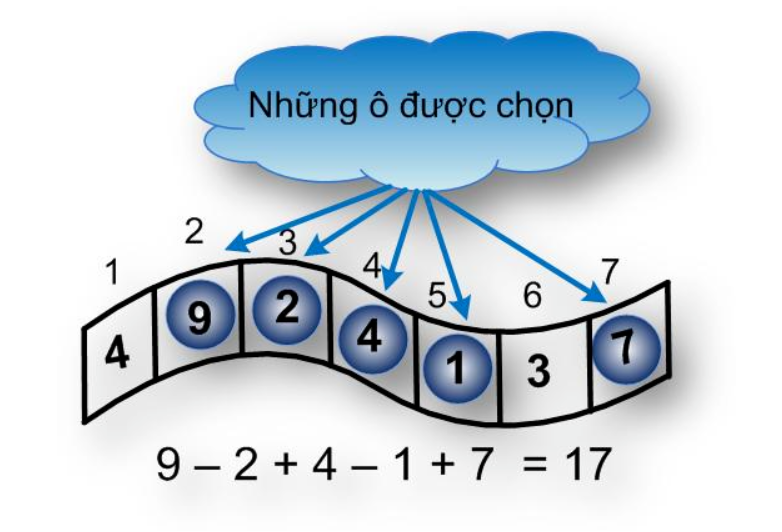
\includegraphics[width=0.5\textwidth]{img/linegame.png}
    \caption{Hình minh họa bài toán.}
\end{figure}

\textbf{Phân tích bài toán}

Gọi $f[i][k]$ là số điểm lớn nhất có thể đạt được khi xét $i$ ô đầu tiên, tại đó $k = 0$ là đặt dấu $+$, $k = 1$ là đặt dấu $-$.

\textbf{Bài toán cơ sở:} $f[1][0] = a[1]$, $f[0][0] = 0$

Xét ô $i$ bất kỳ, ta có các trường hợp có thể xảy ra như sau:

\begin{itemize}
    \item Khi $k = 0$:
    \begin{itemize}
        \item Ta nối với số điểm lớn nhất trước đó khi $k = 1$: $f[i][0] = f[i - 1][1] + a[i]$.
        \item Bắt đầu dãy mới với ô hiện tại là ô đầu tiên: $f[i][0] = a[i]$.
        \item Hoặc bỏ qua ô $i$: $f[i][0] = f[i - 1][0]$.
    \end{itemize}
    \item Khi $k = 1$:
    \begin{itemize}
        \item Ta nối với số điểm lớn nhất trước đó khi $k = 0$: $f[i][1] = f[i - 1][0] - a[i]$.
        \item Hoặc bỏ qua ô $i$: $f[i][1] = f[i - 1][1]$.
        \item Bắt đầu dãy mới với ô hiện tại là ô đầu tiên: $f[i][1] = -a[i]$.
    \end{itemize}
\end{itemize}


%--------------------------
\subsection{Kinh nghiệm (OLP 10\&11 - 2019)}
Link bài: \url{https://lqdoj.edu.vn/problem/twopaths}

\begin{tcolorbox}[
    colback=blue!5,        % màu nền
    colframe=blue!75!black,% màu viền
    title={Đề bài}
]

Hai anh em An và Bình tham gia một trò chơi thám hiểm trên bảng số \textbf{xTremeMaze}.  
Bảng có kích thước $N \times M$ ($N$ dòng và $M$ cột). Các ô trong bảng được đánh số từ trái qua phải và từ trên xuống dưới.\\

Tại mỗi ô của bảng có ghi một số nguyên là số điểm kinh nghiệm mà người chơi sẽ nhận được khi đi vào ô này.  
Cần lưu ý là số điểm tại một số ô có thể là số âm; khi đó, điểm kinh nghiệm của người chơi sẽ bị giảm nếu đi vào ô này.\\

An và Bình bắt đầu tại ô trái trên, vị trí $(1,1)$.  
Mỗi lượt, một người chỉ có thể di chuyển tới ô kề cạnh ngay phía dưới hoặc ô kề cạnh ngay bên phải và không được phép đi ra khỏi bảng.  
Khi đi qua mỗi ô, người chơi nhận được số điểm kinh nghiệm bằng số nguyên ghi ở ô đó.  
Hành trình kết thúc tại ô $(N,M)$.\\

Mục tiêu của trò chơi này là hai anh em đạt được tổng số điểm cao nhất có thể.  
Theo quy định, các ô mà An và Bình đi qua không được phép trùng nhau, ngoại trừ ô bắt đầu $(1,1)$ và ô kết thúc $(N,M)$. \\

Quy ước: giá trị điểm kinh nghiệm tại ô $(1,1)$ và ô $(N,M)$ đều bằng $0$.\\

\textbf{Yêu cầu:} Hãy viết chương trình tính tổng số điểm kinh nghiệm lớn nhất mà An cùng với Bình đạt được.

\end{tcolorbox}

\textbf{Giới hạn}

\begin{itemize}
    \item $2 \leq N, M \leq 200$
    \item Giá trị tuyệt đối của điểm kinh nghiệm tại mỗi ô không vượt quá $100$
    \item Giá trị điểm kinh nghiệm tại ô $(1,1)$ và $(N,M)$ luôn bằng $0$
\end{itemize}

\textbf{Ví dụ}

\begin{table}[h]
    \centering
    \begin{tabular}{|l|r|}
        \hline
        \textbf{Sample Input} & \textbf{Sample Output} \\
        \hline
        \begin{tabular}[c]{@{}l@{}}3 3 \\
        0 2 3 \\
        4 5 6 \\
        7 8 0\end{tabular} & 32 \\
        \hline
    \end{tabular}
\end{table}


\textbf{Phân tích bài toán}

Gọi $f[\text{step}][x_1][x_2]$ là tổng số điểm kinh nghiệm lớn nhất khi An và Bình đã thực hiện $\text{step} = x + y - 2$ bước, trong đó:

- An đang ở vị trí $(x_1, y_1)$ với $y_1 = \text{step} - x_1 + 2$,

- Bình đang ở vị trí $(x_2, y_2)$ với $y_2 = \text{step} - x_2 + 2$.

Vì tổng số bước di chuyển là $\text{step} = n + m - 2$, ta xét lần lượt các bước $\text{step} = 1 \rightarrow n + m - 2$.

Tại mỗi bước, cập nhật giá trị $f[\text{step}][x_1][x_2]$ từ các trạng thái trước đó tương ứng với 4 tổ hợp di chuyển (An/Bình đi xuống hoặc sang phải):

\[
\begin{aligned}
f[\text{step}][x_1][x_2] = \max \Big\{ &f[\text{step} - 1][x_1 - 1][x_2 - 1], \\
                                       &f[\text{step} - 1][x_1 - 1][x_2], \\
                                       &f[\text{step} - 1][x_1][x_2 - 1], \\
                                       &f[\text{step} - 1][x_1][x_2] \Big\} + \text{điểm}
\end{aligned}
\]

Trong đó, phần \textit{điểm} được tính như sau:
\[
\text{nếu } (x_1, y_1) = (x_2, y_2) \Rightarrow \text{điểm} = a[x_1][y_1]
\]
\[
\text{ngược lại} \Rightarrow \text{điểm} = a[x_1][y_1] + a[x_2][y_2]
\]

Ngoài ra, cần đảm bảo các điều kiện sau:
- $(x_1, y_1), (x_2, y_2)$ nằm trong bảng.
- Nếu $(x_1, y_1) = (x_2, y_2)$ thì đó phải là ô đích $(n, m)$.

Kết quả bài toán là: 
\[
\boxed{f[n + m - 2][n][n]}
\]

%-------------------------------------------%
\subsection{IOI07 Miners}
Link bài: \url{https://oj.vnoi.info/problem/nkminers}

\begin{tcolorbox}[
    colback=blue!5,
    colframe=blue!75!black,
    title={Đề bài}
]
Có hai mỏ than, mỗi mỏ có một nhóm thợ mỏ làm việc. Khai thác than là công việc vất vả, do đó các thợ mỏ cần thực phẩm để hoạt động. Mỗi khi một đợt vận chuyển thực phẩm đến mỏ, các thợ mỏ sẽ khai thác được một lượng than nào đó. Có 3 loại thực phẩm được vận chuyển: thịt (M), cá (F) và bánh mì (B).

Mỗi đợt vận chuyển thực phẩm được đưa đến một trong hai mỏ, và sản lượng than của đợt đó phụ thuộc vào số loại thực phẩm khác nhau trong hai đợt liên tiếp mà mỏ đó nhận được:
\begin{itemize}
    \item Nếu các đợt vận chuyển cùng một loại thực phẩm $\Rightarrow$ 1 đơn vị than
    \item Nếu có 2 loại thực phẩm khác nhau $\Rightarrow$ 2 đơn vị than
    \item Nếu có 3 loại thực phẩm khác nhau $\Rightarrow$ 3 đơn vị than
\end{itemize}

Các đợt vận chuyển không thể chia nhỏ, và tất cả thực phẩm trong một đợt phải gửi đến một trong hai mỏ. Có thể gửi tất cả các đợt đến một mỏ.

Hãy tìm cách phân chia các đợt vận chuyển sao cho tổng lượng than khai thác được từ hai mỏ là lớn nhất.
\end{tcolorbox}

\textbf{Giới hạn}
\begin{itemize}
    \item $1 \le N \le 10^5$ - số đợt vận chuyển thực phẩm
    \item Mỗi đợt là một ký tự: M (thịt), F (cá), hoặc B (bánh mì)
\end{itemize}

\textbf{Ví dụ}

\begin{table}[H]
    \centering
    \begin{tabular}{|l|l|}
        \hline
        \textbf{Sample Input} & \textbf{Sample Output} \\
        \hline
        \texttt{6} & \texttt{12} \\
        \texttt{MBMFFB} & \\
        \hline
        \texttt{16} & \texttt{29} \\
        \texttt{MMBMBBBBMMMMMBMB} & \\
        \hline
    \end{tabular}
\end{table}

\textbf{Phân tích bài toán}

Gọi $f[i][a_1][a_2][b_1][b_2]$ là tổng lượng than lớn nhất có thể sản xuất được sau $i$ đợt vận chuyển, trong đó:
\begin{itemize}
    \item $a_1, a_2$ là hai loại thực phẩm gần nhất mỏ 1 đã nhận (Hiện tại là $a_1$, ngày hôm trước là $a_2$).
    \item $b_1, b_2$ là hai loại thực phẩm gần nhất mỏ 2 đã nhận (Hiện tại là $b_1$, ngày hôm trước là $b_2$).
    \item Giá trị của mỗi loại: $0$ (không có), $1$ (M), $2$ (F), $3$ (B).
\end{itemize}

Bài toán cơ sở:

Giả sử thực phẩm đầu tiên là loại $t = \texttt{code}(s[1])$, ta có:
\begin{align*}
f[1][t][0][0][0] &= 1 \quad \text{(gửi đến mỏ 1)} \\
f[1][0][0][t][0] &= 1 \quad \text{(gửi đến mỏ 2)}
\end{align*}

Với $i \geq 2$, giả sử loại thực phẩm hiện tại là $c = \texttt{code}(s[i])$, ta có hai lựa chọn:

\begin{itemize}
    \item \textbf{Chuyển đến mỏ 1}:
    \[
    f[i][c][a_1][b_1][b_2] = \max(f[i][c][a_1][b_1][b_2], f[i - 1][a_1][a_2][b_1][b_2] + \texttt{energy}(c, a_1, a_2))
    \]
    
    \item \textbf{Chuyển đến mỏ 2}:
    \[
    f[i][a_1][a_2][c][b_1] = \max(f[i][a_1][a_2][c][b_1], f[i - 1][a_1][a_2][b_1][b_2] + \texttt{energy}(c, b_1, b_2))
    \]
\end{itemize}

Trong đó, hàm \texttt{energy}(a, b, c) là hàm đếm số loại thực phẩm khác nhau trong 3 ngày gần nhất:
\[
\texttt{energy}(a, b, c) = \left| \{a, b, c\} \setminus \{0\} \right|
\]


Kết quả bài toán:
\[\boxed{
\max(
f[n][a_1][a_2][b_1][b_2], \forall a_1, a_2, b_1, b_2 \in \{0,1,2,3\})}
\]

%--------------------------------------------------$
\subsection{Exam Cheating}
Link bài: \url{https://codeforces.com/problemset/problem/796/E}

\begin{tcolorbox}[
    colback=blue!5,        % màu nền
    colframe=blue!75!black,% màu viền
    title={Đề bài}
]
Zane và người mà Zane thích vừa mới bắt đầu hẹn hò! Tuy nhiên, cô gái đang gặp khó khăn với kỳ thi cuối kỳ môn Vật lý, và cần bạn giúp đỡ.

Có n câu hỏi, được đánh số từ $1$ đến $n$. Câu hỏi $i$ sẽ đứng trước câu hỏi $i + 1$ $(1 \leq i < n)$. Mỗi câu hỏi không thể chọn bừa, vì nếu trả lời sai sẽ bị phạt rất nặng. May mắn thay, cô gái đang ngồi giữa hai thiên tài, và cô ấy sẽ quay cóp bài họ.

Tuy nhiên, hai thiên tài cũng có giới hạn. Mỗi người có thể biết hoặc không biết câu trả lời của một số câu hỏi. Dù vậy, những câu trả lời trên bài của họ thì luôn chính xác tuyệt đối.

Để không bị giám thị phát hiện, cô gái chỉ được quay cóp tối đa $p$ lần, mỗi lần nhìn được nhiều nhất $k$ câu hỏi liên tiếp từ bài của một trong hai thiên tài. Khi cô ấy nhìn vào bài một thiên tài, nếu câu hỏi đó có trong bài của họ, cô ấy sẽ chép lại, nếu không thì bỏ qua.

Nhiệm vụ của bạn là giúp cô ấy trả lời đúng được nhiều nhất bao nhiêu câu hỏi.
\end{tcolorbox}

\textbf{Input Format}

\begin{itemize}
    \item Dòng đầu tiên chứa ba số nguyên $n$, $p$, và $k$ ($1 \leq n, p \leq 1000$, $1 \leq k \leq \min(n, 50)$) - lần lượt là số lượng câu hỏi, số lần quay cóp tối đa, và số lượng câu hỏi liên tiếp tối đa có thể nhìn trong một lần quay cóp.
    \item Dòng thứ hai bắt đầu với một số nguyên $r$ ($0 \leq r \leq n$) - số lượng câu hỏi mà thiên tài thứ nhất có câu trả lời. Tiếp theo là $r$ số nguyên phân biệt $a_1, a_2, \dots, a_r$ ($1 \leq a_i \leq n$), theo thứ tự tăng dần.
    \item Dòng thứ ba bắt đầu với một số nguyên $s$ ($0 \leq s \leq n$) - số lượng câu hỏi mà thiên tài thứ hai có câu trả lời. Tiếp theo là $s$ số nguyên phân biệt $b_1, b_2, \dots, b_s$ ($1 \leq b_i \leq n$), theo thứ tự tăng dần.
\end{itemize}

\textbf{Giới hạn}
\begin{itemize}
    \item $1 \leq n, p \leq 10^3$
    \item $1 \leq k \leq \min(n, 50)$
    \item $0 \leq r, s \leq n$
    \item $1 \leq a_i, b_i \leq n$
    \item Các dãy $a$ và $b$ được sắp xếp tăng dần và không có phần tử trùng nhau.
\end{itemize}

\textbf{Ví dụ}

\begin{table}[h] 
    \centering
    \begin{tabular}{|l|r|}
        \hline
        \textbf{Sample Input} & \textbf{Sample Output} \\
        \hline
        \begin{tabular}[c]{@{}l@{}}%
        6 2 3\\
        3 1 3 6\\
        4 1 2 5 6
        \end{tabular}
        & 4 \\
        \hline
        \begin{tabular}[c]{@{}l@{}}%
        8 3 3\\
        4 1 3 5 6\\
        5 2 4 6 7 8
        \end{tabular}
        & 7 \\
        \hline
    \end{tabular}
\end{table}

\textbf{Ghi chú}

Giả sử $(x, l, r)$ biểu diễn hành động nhìn vào các câu hỏi $i$ sao cho $l \leq i \leq r$ trên bài làm của thiên tài thứ $x$.

Trong ví dụ đầu tiên, cô gái có thể trả lời đúng 4 câu hỏi bằng cách thực hiện các hành động: $(1, 1, 3)$ và $(2, 5, 6)$.

Trong ví dụ thứ hai, cô gái có thể thực hiện các hành động: $(1, 3, 5)$, $(2, 2, 4)$ và $(2, 6, 8)$ để trả lời đúng 7 câu hỏi.\\


\textbf{Phân tích bài toán}

Gọi $f[i][p][g]$ là số câu đúng được nhiều nhất khi làm đến câu $i$, lần gian lận hiện tại là $p$, nhìn bài thiên tài $g$

Bài toán cơ sở:\\

$f[0][p][g] = 0$


%------------------------------------------------------------------------------%
\section{Quy hoạch động nâng cao (Level 2)}

%------------------------------------------------------------------------------%
\section{Quy hoạch động nâng cao (Level 3)}

%------------------------------------------------------------------------------%
\section{Đổi biến số trong quy hoạch động}

%------------------------------------------------------------------------------%
\section{Một số bài tập về đổi biển số}

%------------------------------------------------------------------------------%


\section{Miscellaneous}

\subsection{Contributors}


%------------------------------------------------------------------------------%

\printbibliography[heading=bibintoc]
	
\end{document}